%%%%%%%%%%%%%%%%%%%%%%%%%%%%%%%%%%%%%%%%%%%%%%%%%%%%%%%%%%%%%%%%%%%
%                                                                 %                    
%                 Packages / Grundeinstellungen                   %
%                                                                 %
%%%%%%%%%%%%%%%%%%%%%%%%%%%%%%%%%%%%%%%%%%%%%%%%%%%%%%%%%%%%%%%%%%%
\DocumentMetadata{
    pdfversion=2.0,
    pdfstandard=A-4,
}

\documentclass[paper=a1,parskip=half,fontsize=24]{scrartcl}

\usepackage[ngerman]{babel}
\usepackage{lmodern}
\usepackage{fontspec}
\usepackage{calc}
\usepackage{microtype}
\usepackage{tcolorbox}
\usepackage{blindtext}
\usepackage{float}
\usepackage{subcaption}

% Keine floats in andere Sections
\usepackage[section]{placeins}

% Eurozeichen einbinden
\usepackage[right]{eurosym}

% Floatende Bilder ermöglichen
\usepackage{floatflt}

% Bricht lange URLs "schön" um
\usepackage[hyphens,obeyspaces,spaces]{url}

% Mathematische Symbole importieren
\usepackage{amssymb}

% Zitierung nach APA
%\usepackage[
%backend=biber,
%style=apa,
%autocite=inline,
%]{biblatex}
%\addbibresource{bibtex/poster.bib}

% Zitierung nach IEEE
\usepackage[
backend=biber,
style=ieee,
autocite=inline,
]{biblatex}
\addbibresource{bibtex/poster.bib}

\setcounter{biburllcpenalty}{7000}
\setcounter{biburlucpenalty}{8000}

% Paket für Zeilenabstand
\usepackage{setspace}

% Für Bildbezeichner
\usepackage{capt-of}

% Für Stichwortverzeichnis
\usepackage{makeidx}

% Erzeugt Inhaltsverzeichnis mit Querverweisen zu den Abschnitten (PDF Version)
\usepackage[bookmarksnumbered,hyperfootnotes=false,hypertexnames=false]{hyperref}
\hypersetup{
  colorlinks=true,
  linkcolor=black,
  filecolor=blue,
  citecolor = black,      
  urlcolor=blue,
  }

%mehrspaltig
\usepackage{multicol} 
\columnsep=70pt 
\columnseprule=3pt 

%grafiken einbinden
\usepackage{graphicx}

% Booktabs Tabellen
\usepackage{tabularray}
\UseTblrLibrary{booktabs}
\DefTblrTemplate{contfoot-text}{normal}{Fortsetzung auf nächster Seite}
\SetTblrTemplate{contfoot-text}{normal}
\DefTblrTemplate{conthead-text}{normal}{}
\SetTblrTemplate{conthead-text}{normal}

% Paket für Textfarben
\usepackage{xcolor} 
\definecolor{LightGray}{gray}{0.9}
\usepackage[pagecolor=white]{pagecolor}

% Für schönere Listings
\usepackage[outputdir=log, newfloat,]{minted}
\setminted{
  frame=lines,
  framesep=2mm,
  baselinestretch=1.2,
  bgcolor=LightGray,
  fontsize=\footnotesize,
  linenos,
  breaklines=true,
  breakanywhere=true,
  autogobble,
  tabsize=2
}
\setmintedinline{}

% Keine Floats bei Listings
\newenvironment{code}[2]
  {
  \providecommand{\captiontitle}{#1}
  \providecommand{\labeltitle}{#2}
  \vspace*{0.3cm}
  }
  {
  %\vspace*{-2.0cm}
  \captionbelowof{listing}{\captiontitle}
  \label{\labeltitle}
  \vspace*{0.35cm}
  }
\SetupFloatingEnvironment{listing}{}

%seitengeometrie
\usepackage{geometry}
\geometry{margin=3cm,top=3cm}

%Definition Schrift- und Farbeinstellungen 
\setmainfont{TeX Gyre Termes}
\setsansfont{TeX Gyre Adventor}
\usepackage{preamble}


%Siehe hierzu preamble.sty
\colorlet{basecolor}{meerblau}
\colorlet{akzentcolor}{mint}

%Siehe hierzu preamble.sty
%\renewcommand{\theauthor}{Thore Hüneke thohueneke, Anette Michlik anemichlik, Kasem Rashrash kasrashrash, Sophie Sergeenko sopsergeenko}
%\renewcommand{\thetitle}{Impftermine digital: Schnell. Sicher. Skalierbar.}
%\renewcommand{\thesubtitle}{Von der technischen Umsetzung zur Qualitätssicherung}

%Höhe des HS Logos 4cm für zweizeiligen Titel, 2.5cm für einzeiligen Titel
\newcommand{\myspace}{4cm}

\hypersetup{pdfinfo={
  Title={\thetitle},
  Author={\theauthor}
}}

% Darf erst hier eingebunden werden! 
\usepackage{csquotes}

%Textfarbe
\color{black}

%%%%%%%%%%%%%%%%%%%%%%%%%%%%%%%%%%%%%%%%%%%%%%%%%%%%%%%%%%%%%%%%%%%
%                                                                 %                    
%                     Beginn des Inhalts                          %
%                                                                 %
%%%%%%%%%%%%%%%%%%%%%%%%%%%%%%%%%%%%%%%%%%%%%%%%%%%%%%%%%%%%%%%%%%%

%%%%%%%%%%%%%%%%%%%%%%%%%%%%%%%%%%%%%%%%%%%%%%%%%%%%%%%%%%%%%%%%%%%
%  Special Characters:                                            %
%                                                                 %
%             \& \% \$ \# \_ \{ \}                                %
%             \textasciitilde (~)                                 %
%             \textasciicircum (^)                                %     
%             \textbackslash (\)                                  %                    
%      \glqq Text\grqq{} für Anführungszeichen                    %
%%%%%%%%%%%%%%%%%%%%%%%%%%%%%%%%%%%%%%%%%%%%%%%%%%%%%%%%%%%%%%%%%%%


\begin{document}
  %Printed Überschriften
  %\thetitlearea
  %Mehrspaltig
  \begin{multicols*}{3}
  
    % Input Inhalt
    \section*{Qualitätssicherung}

Qualitätssicherung ist ein zentraler Bestandteil in der Softwareentwicklung, um sicherzustellen, dass das System zuverlässig, sicher und effizient arbeitet. Sie hilft dabei, Fehler frühzeitig zu erkennen und zu beseitigen sowie Risiken zu minimieren.
Für Stabilität und Sicherheit sorgen wir durch systematische Tests, Versionskontrolle mittels Git und automatisierte Prozesse (DevOps). 
Wir führen unterschiedliche Tests durch, um Fehler frühzeitig zu entdecken und zu beheben.
Mittels Git-Versionierung und CI/CD-Pipelines automatisieren wir den Integrations- und Deploymentprozess, wodurch die Software stets stabil und schnell bereitgestellt werden kann. Durch Lasttests überprüfen wir die Leistungsfähigkeit und Skalierbarkeit des Systems unter verschiedenen Bedingungen. Ergebnisse werden ausgewertet und optimiert, um die Systemstabilität und Sicherheit langfristig zu gewährleisten.


    \section*{DevOps}

\textbf{Wie wird das System versioniert & bereitgestellt?}

Unser System wird mithilfe von Git versioniert. Änderungen im Quellcode werden zentral über Git verwaltet, und bei jedem Push auf das Repository erfolgt eine automatische Ausführung von Skripten zur Bereitstellung. Wir verwenden hauptsächlich einen einzigen Branch (main). Neue Änderungen werden dort gesammelt.
In unserem System verwenden wir auch Git-Hooks. Das bedeutet, dass nach jeder Änderung automatisch geprüft wird, 
ob der Code Fehler enthält und verschiedene Prozesse gestartet werden. 
Die Integration des CI/CD-Prozesses erfolgt mittels Git post-receive-Hook. Bei einem Push auf den main-Branch lädt er zunächst die Konfigurationsdatei und startet anschließend den automatischen Build mit dem Skript build.sh. Danach erfolgt ein automatisierter Login-Vorgang mittels einer HTTP-Anfrage (curl) an unsere Anwendung. Somit realisiert der post-receive einen kontinuierlichen Deployment-Prozess.
Was die Lizenz angeht, wurde die \textbf{MIT-Lizenz} gewählt, weil sie eine Open-Source-Lizenz ist. Außerdem ist sie einfach und flexibil, da sie sehr liberal ist und anderen Entwicklern erlaubt, den Code leicht weiterzuverwenden und anzupassen.

\textbf{Post-receive Hook}
\begin{lstlisting}[language=bash]
#!/bin/bash

configfile="/home/$USER/repos/swe3-2024-03/local/config.txt"

while read oldrev newrev refname
do
  ...

  branch=$(echo "$refname" | sed 's|^refs/heads/||')
  if [ "$branch" = "main" ]; then
    echo "Starte Deployment für main..."

  if test "$configfile" != ""; then
    source "$configfile"
  fi

   cd ~/repos/swe3-2024-03/ || exit 1
   bin/build.sh
  fi
done

exit 0
\end{lstlisting}

\textbf{Pre-receive Hook}
\begin{lstlisting}[language=bash]
#!/bin/bash

while read oldrev newrev refname
do
 ... 

 find "$tmpdir" -name '*.java' \
       | xargs -r -n 1000 google-java-format --set-exit-if-changed
  formatter_status=$?
  if [ $formatter_status -ne 0 ]; then
    echo "Fehler: google-java-formatter."
    exit 1

find "$tmpdir" -name '*.java' \
     | xargs -r -n 1000 checkstyle -c ~/repos/swe3-2024-03/misc/checkstyle.xml
status=$?
if [ $status -ne 0 ]; then
  echo "Checkstyle Fehlermeldung"
  rm -rf "$tmpdir"
  exit 1
fi
  rm -rf "$tmpdir"

done

exit 0
\end{lstlisting}

\textbf{Commit-msg}
\begin{lstlisting}[language=bash]
#!/bin/bash

COMMIT_MSG_FILE="$1"
COMMIT_MSG=$(cat "$COMMIT_MSG_FILE")

REGEX='^(ADD|DELETE|CHANGE)\s*\|\s*[^|]+\s*\|\s*.*$'

if [[ ! "$COMMIT_MSG" =~ $REGEX ]]; then
    echo "ERROR: Format nicht eingehalten!"
    echo "AUFGABE(ADD,DELETE,CHANGE) | DATEINAME | NACHRICHT"
    exit 1
fi

exit 0
\end{lstlisting}

    \section*{1000-Servlets}
\textbf{Experiment mit 1000 Servlets}

In diesem Experiment haben wir 1000 neue Servlet-Dateien 
(\texttt{Servlet1.java} bis \texttt{Servlet1000.java}) in das Repository 
hochgeladen, was insgesamt 13.000 neue Codezeilen umfasste.
Zunächst haben wir mithilfe von \texttt{xargs} pro Aufruf nur 50 Dateien an 
Checkstyle und den Google Java Formatter übergeben. Dabei ergab sich eine hohe 
Wartezeit von etwa \textbf{24,6 Sekunden}, was für 1000 Dateien sehr lang ist.  
Da ein Push abgelehnt wird, sobald Checkstyle Fehler findet, war diese Verzögerung problematisch.
Um die Performance zu verbessern, haben wir unsere Aufrufe angepasst:  
Statt 50 Dateien pro Durchgang übergaben wir nun alle 1000 Dateien auf einmal.  
Zusätzlich wurden nur die \textbf{geänderten} Servlets geprüft, anstatt alle erneut zu analysieren.
\paragraph{Ergebnis:}
\begin{itemize}
    \item \textbf{Vorher:} 24,6 Sekunden (bei \texttt{xargs -n 50})
    \item \textbf{Jetzt:} 10,6 Sekunden (bei \texttt{xargs -n 1000})
\end{itemize}

Die Zeit konnte somit um rund \textbf{60 Prozent} reduziert werden.  
Negative Auswirkungen auf CPU- oder RAM-Auslastung waren nicht zu beobachten.  
Falls dennoch weitere Verzögerungen auftreten, könnte das Netzwerk der Flaschenhals sein.  
Die minimalen \texttt{user} und \texttt{sys}-Zeiten deuten darauf hin, dass die Hauptverzögerung 
auf I/O- und Netzwerkprozesse zurückzuführen ist.
Durch die Verringerung der Checkstyle-Aufrufe (von rund 20 auf 1) hat sich die Push-Zeit 
\textbf{mehr als halbiert}.  
Dieses Experiment zeigt, dass Checkstyle effizienter arbeitet,  
wenn eine große Liste an Dateien in einem Durchgang geprüft wird,  
anstatt viele kleine Prozesse zu starten.  
So konnten wir erfolgreich untersuchen, wie das Repository und der Hook unter Einfluss 
von Checkstyle und Google Java Formatter mit einer großen Anzahl neuer Dateien umgehen.


    \section*{Testfälle}

\FloatBarrier % Verhindert, dass die Tabelle verschoben wird

\begin{table}[H] % Nutze H statt h!
    \centering
   % \tiny
    \scriptsize
    \renewcommand{\arraystretch}{1.2}
    \begin{tabular}{|p{3cm}|p{7.9cm}|p{6.7cm}|}
        \hline
        \textbf{Testfall} & \textbf{Eingabe} & \textbf{Erwartetes Ergebnis} \\ \hline

        Registrierung (erfolgreich) &
        \parbox{6cm}{
          \texttt{curl -X POST -d} \\
          \texttt{"email=testuser@example.com\&} \\
          \texttt{password=123\&} \\
          \texttt{passwordConfirm=123"} \\
          \texttt{\$path/register}
        } &
        \texttt{"message": "Registrierung erfolgreich!", Status: success} \\ \hline

        Registrierung (Fehlgeschlagen) &
        \parbox{6cm}{
          \texttt{curl -X POST -d} \\
          \texttt{"email=testuser@example.com\&} \\
          \texttt{password=123"} \\
          \texttt{\$path/register}
        } &
        \texttt{"message": "E-Mail bereits registriert.", status: error} \\ \hline

        Login (erfolgreich) &
        \parbox{6cm}{
          \texttt{curl -X POST -c cookie -b cookie -d} \\
          \texttt{"email=testuser@example.com\&} \\
          \texttt{password=123"} \\
          \texttt{\$path/UserAnmelden}
        } &
        \texttt{"redirect": "termine", "message": "Login erfolgreich", status: success} \\ \hline

        Session prüfen &
        \parbox{6cm}{
          \texttt{curl -b cookie \$path/SessionPruefen}
        } &
        Session gültig – JSON mit Benutzerdaten oder Status \\ \hline

        Freie Slots anzeigen &
        \parbox{6cm}{
          \texttt{curl -X POST -b cookie \$path/FreieSlotsAnzeigen}
        } &
        Liste der verfügbaren Slots im JSON-Format \\ \hline

        Impfstoffe abrufen &
        \parbox{6cm}{
          \texttt{curl -b cookie} \\
          \texttt{"\$path/ImpfstoffAnzeigen?} \\
          \texttt{impfzentren=Nemerb-Nord"} \\
        } &
        Liste der Impfstoffe als JSON \\ \hline

        Termin buchen &
        \parbox{6cm}{
          \texttt{curl -X POST -b cookie -d} \\
          \texttt{"datum=2025-03-20\&zeit=08:30\&} \\
          \texttt{impfstoff\_id=1\&} \\
          \texttt{impfzentrum=Nemerb-Nord"} \\
          \texttt{\$path/TerminBuchen}
        } &
        \texttt{"message": "Termin erfolgreich gebucht", status : success} \\ \hline

        Buchungen anzeigen &
        \parbox{6cm}{
          \texttt{curl -b cookie \$path/BuchungAnzeigen}
        } &
        JSON mit allen Buchungen des Nutzers \\ \hline

        Termin stornieren &
        \parbox{6cm}{
          \texttt{curl -X POST -b cookie -d} \\
          \texttt{"buchung\_id=1"} \\
          \texttt{\$path/TerminStornieren}
        } &
        \texttt{"message": "Buchung erfolgreich gelöscht", status: success} \\ \hline

        Logout &
        \parbox{6cm}{
          \texttt{curl -X POST -b cookie \$path/UserAbmelden}
        } &
        \texttt{"message": "Abmeldung erfolgreich", status: success} \\ \hline

        Zugriff nach Logout &
        \parbox{6cm}{
          \texttt{curl -b cookie \$path/SessionPruefen}
        } &
        \texttt{"message": "Keine aktive Session", status: error} \\ \hline

    \end{tabular}
    \caption{Testfälle für die Impfregistrierungsanwendung}
    \label{tab:testfaelle}
\end{table}

\FloatBarrier % Sicherstellen, dass nichts weiter nach unten rutscht


    \section*{Performanceanalyse}

\begin{center}
  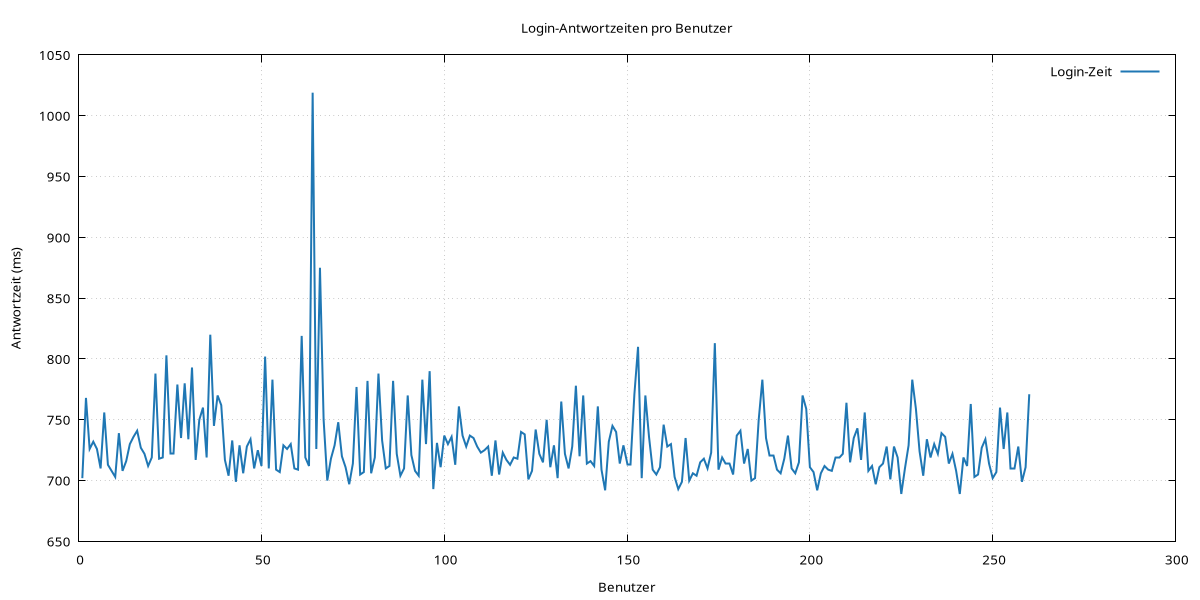
\includegraphics[width=0.95\linewidth, height=0.45\textheight, keepaspectratio]{src/abbildungen/login_lasttest.png}
  \captionof{figure}{Lasttest}
\end{center}

In unserem Lasttest wurden Login-Antwortzeiten mit steigender Benutzeranzahl gemessen. 
Für diesen Test wurden in Gruppen von 10, 25, 50, 75 und 100 Benutzern jeweils neue Testnutzer automatisch registriert und anschließend eingeloggt. Jeder Login wurde mit curl per HTTP-POST-Anfrage durchgeführt, wobei die Antwortzeit in Millisekunden 
sowie der HTTP-Statuscode erfasst wurde. Das Ziel war es, die Skalierbarkeit und Belastbarkeit des Systems im Bereich „Login“ zu analysieren, insbesondere unter der Annahme, dass bei hohem Nutzeraufkommen (wie in Pandemiesituationen) viele Benutzer innerhalb kurzer Zeit gleichzeitig auf das System zugreifen.

    \section*{Ausblick}

Weiterentwicklung 
Übergabe an weitere Behörden
Weitere Optimierungsmöglichkeiten
Eventuelle Erweiterungen (z. B. mobile App, bessere UI)

Reflexion 
Was hat gut funktioniert?
Wo gab es Herausforderungen?


    
    % Literaturverzeichnis anzeigen
    \section*{Referenzen}
    \vspace*{0.3cm}
    \nocite{*}
    \printbibliography[heading=none]

  \end{multicols*}
\end{document}

